% Options for packages loaded elsewhere
\PassOptionsToPackage{unicode}{hyperref}
\PassOptionsToPackage{hyphens}{url}
\PassOptionsToPackage{dvipsnames,svgnames,x11names}{xcolor}
%
\documentclass[
  letterpaper,
  DIV=11,
  numbers=noendperiod,
  oneside]{scrartcl}

\usepackage{amsmath,amssymb}
\usepackage{iftex}
\ifPDFTeX
  \usepackage[T1]{fontenc}
  \usepackage[utf8]{inputenc}
  \usepackage{textcomp} % provide euro and other symbols
\else % if luatex or xetex
  \usepackage{unicode-math}
  \defaultfontfeatures{Scale=MatchLowercase}
  \defaultfontfeatures[\rmfamily]{Ligatures=TeX,Scale=1}
\fi
\usepackage{lmodern}
\ifPDFTeX\else  
    % xetex/luatex font selection
\fi
% Use upquote if available, for straight quotes in verbatim environments
\IfFileExists{upquote.sty}{\usepackage{upquote}}{}
\IfFileExists{microtype.sty}{% use microtype if available
  \usepackage[]{microtype}
  \UseMicrotypeSet[protrusion]{basicmath} % disable protrusion for tt fonts
}{}
\makeatletter
\@ifundefined{KOMAClassName}{% if non-KOMA class
  \IfFileExists{parskip.sty}{%
    \usepackage{parskip}
  }{% else
    \setlength{\parindent}{0pt}
    \setlength{\parskip}{6pt plus 2pt minus 1pt}}
}{% if KOMA class
  \KOMAoptions{parskip=half}}
\makeatother
\usepackage{xcolor}
\usepackage[left=1in,marginparwidth=2.0666666666667in,textwidth=4.1333333333333in,marginparsep=0.3in]{geometry}
\setlength{\emergencystretch}{3em} % prevent overfull lines
\setcounter{secnumdepth}{-\maxdimen} % remove section numbering
% Make \paragraph and \subparagraph free-standing
\ifx\paragraph\undefined\else
  \let\oldparagraph\paragraph
  \renewcommand{\paragraph}[1]{\oldparagraph{#1}\mbox{}}
\fi
\ifx\subparagraph\undefined\else
  \let\oldsubparagraph\subparagraph
  \renewcommand{\subparagraph}[1]{\oldsubparagraph{#1}\mbox{}}
\fi

\usepackage{color}
\usepackage{fancyvrb}
\newcommand{\VerbBar}{|}
\newcommand{\VERB}{\Verb[commandchars=\\\{\}]}
\DefineVerbatimEnvironment{Highlighting}{Verbatim}{commandchars=\\\{\}}
% Add ',fontsize=\small' for more characters per line
\usepackage{framed}
\definecolor{shadecolor}{RGB}{241,243,245}
\newenvironment{Shaded}{\begin{snugshade}}{\end{snugshade}}
\newcommand{\AlertTok}[1]{\textcolor[rgb]{0.68,0.00,0.00}{#1}}
\newcommand{\AnnotationTok}[1]{\textcolor[rgb]{0.37,0.37,0.37}{#1}}
\newcommand{\AttributeTok}[1]{\textcolor[rgb]{0.40,0.45,0.13}{#1}}
\newcommand{\BaseNTok}[1]{\textcolor[rgb]{0.68,0.00,0.00}{#1}}
\newcommand{\BuiltInTok}[1]{\textcolor[rgb]{0.00,0.23,0.31}{#1}}
\newcommand{\CharTok}[1]{\textcolor[rgb]{0.13,0.47,0.30}{#1}}
\newcommand{\CommentTok}[1]{\textcolor[rgb]{0.37,0.37,0.37}{#1}}
\newcommand{\CommentVarTok}[1]{\textcolor[rgb]{0.37,0.37,0.37}{\textit{#1}}}
\newcommand{\ConstantTok}[1]{\textcolor[rgb]{0.56,0.35,0.01}{#1}}
\newcommand{\ControlFlowTok}[1]{\textcolor[rgb]{0.00,0.23,0.31}{#1}}
\newcommand{\DataTypeTok}[1]{\textcolor[rgb]{0.68,0.00,0.00}{#1}}
\newcommand{\DecValTok}[1]{\textcolor[rgb]{0.68,0.00,0.00}{#1}}
\newcommand{\DocumentationTok}[1]{\textcolor[rgb]{0.37,0.37,0.37}{\textit{#1}}}
\newcommand{\ErrorTok}[1]{\textcolor[rgb]{0.68,0.00,0.00}{#1}}
\newcommand{\ExtensionTok}[1]{\textcolor[rgb]{0.00,0.23,0.31}{#1}}
\newcommand{\FloatTok}[1]{\textcolor[rgb]{0.68,0.00,0.00}{#1}}
\newcommand{\FunctionTok}[1]{\textcolor[rgb]{0.28,0.35,0.67}{#1}}
\newcommand{\ImportTok}[1]{\textcolor[rgb]{0.00,0.46,0.62}{#1}}
\newcommand{\InformationTok}[1]{\textcolor[rgb]{0.37,0.37,0.37}{#1}}
\newcommand{\KeywordTok}[1]{\textcolor[rgb]{0.00,0.23,0.31}{#1}}
\newcommand{\NormalTok}[1]{\textcolor[rgb]{0.00,0.23,0.31}{#1}}
\newcommand{\OperatorTok}[1]{\textcolor[rgb]{0.37,0.37,0.37}{#1}}
\newcommand{\OtherTok}[1]{\textcolor[rgb]{0.00,0.23,0.31}{#1}}
\newcommand{\PreprocessorTok}[1]{\textcolor[rgb]{0.68,0.00,0.00}{#1}}
\newcommand{\RegionMarkerTok}[1]{\textcolor[rgb]{0.00,0.23,0.31}{#1}}
\newcommand{\SpecialCharTok}[1]{\textcolor[rgb]{0.37,0.37,0.37}{#1}}
\newcommand{\SpecialStringTok}[1]{\textcolor[rgb]{0.13,0.47,0.30}{#1}}
\newcommand{\StringTok}[1]{\textcolor[rgb]{0.13,0.47,0.30}{#1}}
\newcommand{\VariableTok}[1]{\textcolor[rgb]{0.07,0.07,0.07}{#1}}
\newcommand{\VerbatimStringTok}[1]{\textcolor[rgb]{0.13,0.47,0.30}{#1}}
\newcommand{\WarningTok}[1]{\textcolor[rgb]{0.37,0.37,0.37}{\textit{#1}}}

\providecommand{\tightlist}{%
  \setlength{\itemsep}{0pt}\setlength{\parskip}{0pt}}\usepackage{longtable,booktabs,array}
\usepackage{calc} % for calculating minipage widths
% Correct order of tables after \paragraph or \subparagraph
\usepackage{etoolbox}
\makeatletter
\patchcmd\longtable{\par}{\if@noskipsec\mbox{}\fi\par}{}{}
\makeatother
% Allow footnotes in longtable head/foot
\IfFileExists{footnotehyper.sty}{\usepackage{footnotehyper}}{\usepackage{footnote}}
\makesavenoteenv{longtable}
\usepackage{graphicx}
\makeatletter
\def\maxwidth{\ifdim\Gin@nat@width>\linewidth\linewidth\else\Gin@nat@width\fi}
\def\maxheight{\ifdim\Gin@nat@height>\textheight\textheight\else\Gin@nat@height\fi}
\makeatother
% Scale images if necessary, so that they will not overflow the page
% margins by default, and it is still possible to overwrite the defaults
% using explicit options in \includegraphics[width, height, ...]{}
\setkeys{Gin}{width=\maxwidth,height=\maxheight,keepaspectratio}
% Set default figure placement to htbp
\makeatletter
\def\fps@figure{htbp}
\makeatother
\newlength{\cslhangindent}
\setlength{\cslhangindent}{1.5em}
\newlength{\csllabelwidth}
\setlength{\csllabelwidth}{3em}
\newlength{\cslentryspacingunit} % times entry-spacing
\setlength{\cslentryspacingunit}{\parskip}
\newenvironment{CSLReferences}[2] % #1 hanging-ident, #2 entry spacing
 {% don't indent paragraphs
  \setlength{\parindent}{0pt}
  % turn on hanging indent if param 1 is 1
  \ifodd #1
  \let\oldpar\par
  \def\par{\hangindent=\cslhangindent\oldpar}
  \fi
  % set entry spacing
  \setlength{\parskip}{#2\cslentryspacingunit}
 }%
 {}
\usepackage{calc}
\newcommand{\CSLBlock}[1]{#1\hfill\break}
\newcommand{\CSLLeftMargin}[1]{\parbox[t]{\csllabelwidth}{#1}}
\newcommand{\CSLRightInline}[1]{\parbox[t]{\linewidth - \csllabelwidth}{#1}\break}
\newcommand{\CSLIndent}[1]{\hspace{\cslhangindent}#1}

\KOMAoption{captions}{tableheading}
\makeatletter
\makeatother
\makeatletter
\makeatother
\makeatletter
\@ifpackageloaded{caption}{}{\usepackage{caption}}
\AtBeginDocument{%
\ifdefined\contentsname
  \renewcommand*\contentsname{Table of contents}
\else
  \newcommand\contentsname{Table of contents}
\fi
\ifdefined\listfigurename
  \renewcommand*\listfigurename{List of Figures}
\else
  \newcommand\listfigurename{List of Figures}
\fi
\ifdefined\listtablename
  \renewcommand*\listtablename{List of Tables}
\else
  \newcommand\listtablename{List of Tables}
\fi
\ifdefined\figurename
  \renewcommand*\figurename{Figure}
\else
  \newcommand\figurename{Figure}
\fi
\ifdefined\tablename
  \renewcommand*\tablename{Table}
\else
  \newcommand\tablename{Table}
\fi
}
\@ifpackageloaded{float}{}{\usepackage{float}}
\floatstyle{ruled}
\@ifundefined{c@chapter}{\newfloat{codelisting}{h}{lop}}{\newfloat{codelisting}{h}{lop}[chapter]}
\floatname{codelisting}{Listing}
\newcommand*\listoflistings{\listof{codelisting}{List of Listings}}
\makeatother
\makeatletter
\@ifpackageloaded{caption}{}{\usepackage{caption}}
\@ifpackageloaded{subcaption}{}{\usepackage{subcaption}}
\makeatother
\makeatletter
\@ifpackageloaded{tcolorbox}{}{\usepackage[skins,breakable]{tcolorbox}}
\makeatother
\makeatletter
\@ifundefined{shadecolor}{\definecolor{shadecolor}{rgb}{.97, .97, .97}}
\makeatother
\makeatletter
\makeatother
\makeatletter
\@ifpackageloaded{sidenotes}{}{\usepackage{sidenotes}}
\@ifpackageloaded{marginnote}{}{\usepackage{marginnote}}
\makeatother
\makeatletter
\makeatother
\makeatletter
\@ifpackageloaded{fontawesome5}{}{\usepackage{fontawesome5}}
\makeatother
\ifLuaTeX
  \usepackage{selnolig}  % disable illegal ligatures
\fi
\IfFileExists{bookmark.sty}{\usepackage{bookmark}}{\usepackage{hyperref}}
\IfFileExists{xurl.sty}{\usepackage{xurl}}{} % add URL line breaks if available
\urlstyle{same} % disable monospaced font for URLs
\hypersetup{
  pdftitle={1. Introduction},
  colorlinks=true,
  linkcolor={blue},
  filecolor={Maroon},
  citecolor={Blue},
  urlcolor={Blue},
  pdfcreator={LaTeX via pandoc}}

\title{1. Introduction}
\author{}
\date{}

\begin{document}
\maketitle
\ifdefined\Shaded\renewenvironment{Shaded}{\begin{tcolorbox}[interior hidden, breakable, boxrule=0pt, enhanced, frame hidden, borderline west={3pt}{0pt}{shadecolor}, sharp corners]}{\end{tcolorbox}}\fi

\renewcommand{\vec}[1]{\boldsymbol{\mathbf{#1}}}

\newcommand{\Set}[1]{\mathbb{#1}}
\DeclareMathOperator{\erf}{erf} 
\DeclareMathOperator{\sgn}{sgn}

\newcommand{\num}[1]{#1}
\newcommand{\SI}[2]{#1\,\mathrm{#2}}
\newcommand{\SIrange}[3]{#1\,\text{ to }\,#2\,\mathrm{#3}}
\newcommand{\si}[1]{\,\mathrm{#1}}

\newcommand{\per}{/}

\newcommand{\metre}{m}
\newcommand{\second}{s}
\newcommand{\minute}{min}
\newcommand{\hour}{h}
\newcommand{\day}{d}
\newcommand{\kelvin}{K}
\newcommand{\joule}{J}
\newcommand{\gram}{g}
\newcommand{\watt}{W}
\newcommand{\percent}{\%}
\newcommand{\electronvolt}{eV}
\newcommand{\mole}{mol}

\newcommand{\centi}{c}
\newcommand{\kilo}{k}

\newcommand{\tothe}[1]{^{\mathrm{#1}}}
\newcommand{\squared}{\tothe{2}}
\newcommand{\cubed}{\tothe{3}}

\newcommand{\gls}[1]{\text{#1}}
\newcommand{\glspl}[1]{\mathrm{#1's}}

\newcommand{\activationEnergy}{E_a}
\newcommand{\area}{A}
\newcommand{\azimuthAngle}{\vartheta}
\newcommand{\baseVector}{\hat{\vec{e}}}
\newcommand{\cartesianCoordinate}{\vec{x}}
    \newcommand{\cartesianCoordinateX}{x}
    \newcommand{\cartesianCoordinateY}{y}
    \newcommand{\cartesianCoordinateZ}{z}
    \newcommand{\cartesianCoordinateDef}{\left[\cartesianCoordinateX, \cartesianCoordinateY, \cartesianCoordinateZ\right]^T}
    \newcommand{\cartesianBaseVectorX}{\baseVector_\cartesianCoordinateX}
    \newcommand{\cartesianBaseVectorY}{\baseVector_\cartesianCoordinateY}
    \newcommand{\cartesianBaseVectorZ}{\baseVector_\cartesianCoordinateZ}
\newcommand{\density}{\rho}
\newcommand{\distance}{d}
\newcommand{\eccentricity}{e}
\newcommand{\eccentricAnomaly}{E} 
\newcommand{\energy}{E}
    \newcommand{\kineticEnergy}{\energy_{kin}}
    \newcommand{\relativeEnergy}{\epsilon}
    \newcommand{\relativeKineticEnergy}{\relativeEnergy_{kin}}
\newcommand{\error}{e}
\newcommand{\extinctionCoefficient}{E}
\newcommand{\force}{F}
\newcommand{\height}{h}
\newcommand{\latitude}{\Phi}
\newcommand{\localTime}{\Time_\text{LT}}
\newcommand{\longitude}{\Theta}
\newcommand{\machineAccuracy}{\epsilon}
\newcommand{\mass}{m}
\newcommand{\mean}{\mu}
    \newcommand{\meanof}[1]{\langle #1 \rangle}
\newcommand{\meanAnomaly}{M}
\newcommand{\numberDensity}{n}
    \newcommand{\surfaceNumberDensity}{n_0}
\newcommand{\partitionFunction}{\zeta}
\newcommand{\period}{P}
\newcommand{\poissonRatio}{\nu}
\newcommand{\porosity}{\Psi}
\newcommand{\potential}{U}
\newcommand{\pressure}{p}
\newcommand{\radius}{r}
\newcommand{\rate}{k}
\newcommand{\residenceTime}{\tau}
\newcommand{\semiLatusRectum}{p}
\newcommand{\semiMajorAxis}{a}
\newcommand{\source}{s}
\newcommand{\sphericalCoordinate}{\vec{r}}
    \newcommand{\sphericalCoordinateRadius}{r}
    \newcommand{\sphericalCoordinateAzimuth}{\azimuthAngle}
    \newcommand{\sphericalCoordinateElevation}{\varphi}
    \newcommand{\sphericalCoordinateDef}{\left[\sphericalCoordinateRadius, \sphericalCoordinateAzimuth, \sphericalCoordinateElevation\right]^T}
    \newcommand{\sphericalBaseVectorRadius}{\baseVector_\sphericalCoordinateRadius}
    \newcommand{\sphericalBaseVectorAzimuth}{\baseVector_\sphericalCoordinateAzimuth}
    \newcommand{\sphericalBaseVectorElevation}{\baseVector_\sphericalCoordinateElevation}
\newcommand{\standardDeviation}{\sigma}
\newcommand{\sublimationFlux}{\Phi}
\newcommand{\temperature}{T}
\newcommand{\thermalAccommodationCoefficient}{\alpha}
\newcommand{\thermalConductivity}{\lambda}
\newcommand{\Time}{t}
    \newcommand{\flightTime}{\Time_{flight}}
\newcommand{\trueAnomaly}{\theta}
\newcommand{\variance}{\standardDeviation^2}
\newcommand{\velocity}{v}
    \newcommand{\Velocity}{V}
\newcommand{\volume}{V}
\newcommand{\weight}{w}
\newcommand{\youngsModulus}{Y}
\newcommand{\zenithAngle}{\psi}

\newcommand{\BoltzmannConstant}{k_B}
\newcommand{\BoltzmannConstantValue}{\SI{1.38e-23}{\joule\per\kelvin}}
\newcommand{\GasConstant}{R}

\newcommand{\GravitationalConstant}{G}
\newcommand{\GravitationalConstantValue}{\SI{6.674e-11}{\metre\cubed\per\kilo\gram\per\second\squared}}
\newcommand{\StefanBoltzmannConstant}{\sigma}
\newcommand{\StefanBoltzmannConstantValue}{\SI{5.67e-8}{\watt\per\metre\squared\per\kelvin\tothe{4}}}
\newcommand{\PlanckConstant}{h}
\newcommand{\PlanckConstantValue}{\SI{6.626e-34}{\metre\squared\kilo\gram\per\second}}

\begin{center}\rule{0.5\linewidth}{0.5pt}\end{center}

Space exploration has always captivated humanity's imagination, driving
scientific inquiry and technological advancement to unprecedented
heights. While the Moon's surface has been a focal point of human
exploration, its tenuous exosphere, a fragile envelope of particles and
gases, has long remained an understudied frontier. Recent decades have
witnessed remarkable strides in our understanding of extraterrestrial
exospheres, with a particular focus on the Moon's exosphere and its
intricate interactions with the lunar surface.

\begin{figure*}

\section{\texorpdfstring{\faIcon{image} Figure}{ Figure}}

\begin{figure}

\begin{minipage}[t]{0.50\linewidth}

{\centering 

\raisebox{-\height}{

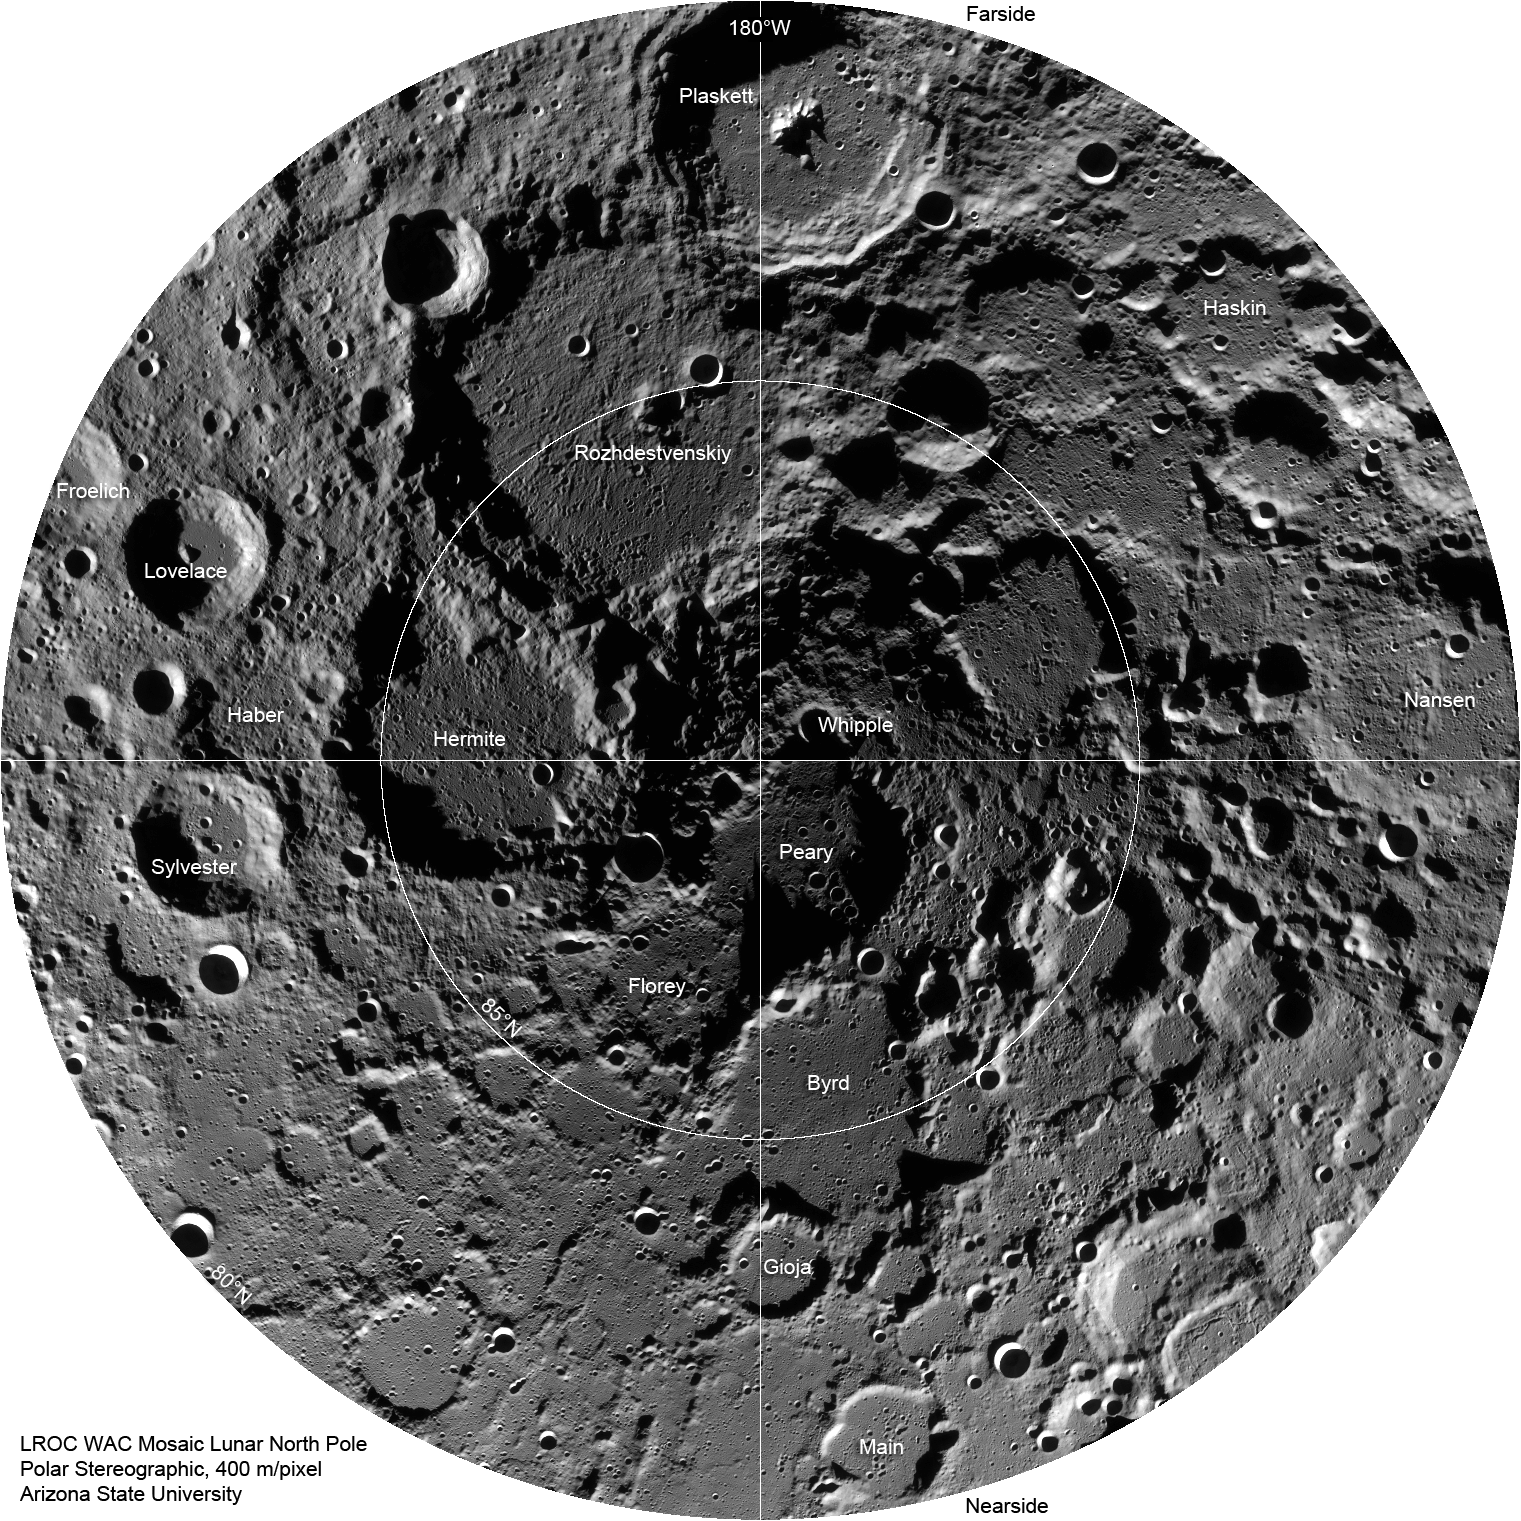
\includegraphics{imgs/LROC_poles/LROC_north_pole.jpg}

}

}

\subcaption{\label{fig-LROC_north_pole}Lunar north pole.}
\end{minipage}%
%
\begin{minipage}[t]{0.50\linewidth}

{\centering 

\raisebox{-\height}{

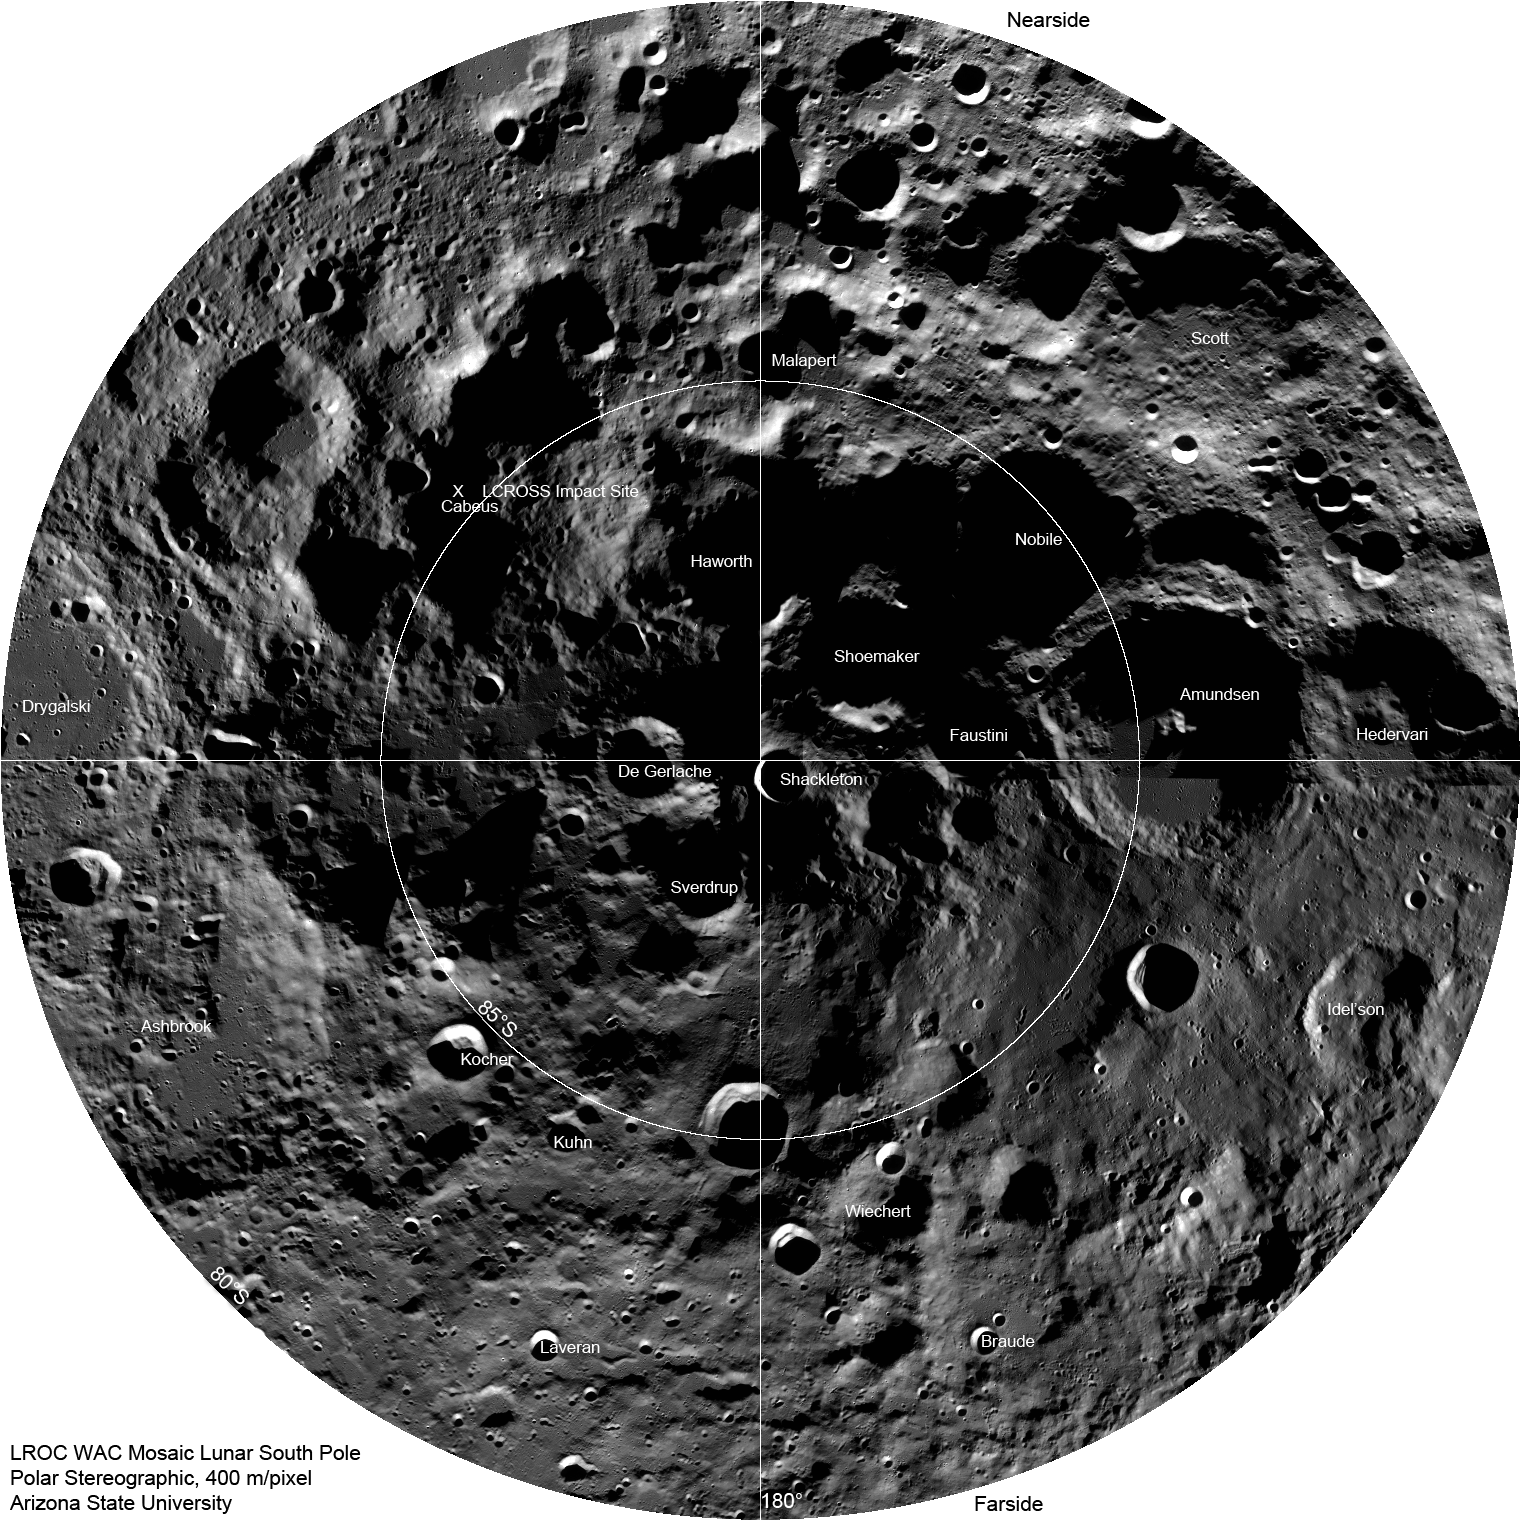
\includegraphics{imgs/LROC_poles/LROC_south_pole.jpg}

}

}

\subcaption{\label{fig-LROC_south_pole}Lunar south pole.}
\end{minipage}%

\caption{\label{fig-LROC_poles}\href{/documentation/acronyms.qmd}{LROC}
Wide Angle Camera (\href{/documentation/acronyms.qmd}{WAC}) mosaic of
the lunar north and south pole region. With a resolution of 400m/pixel,
the total width of each image extends to \textasciitilde600km, ranging
from 80° to 90° latitude, north and south, respectively. The names of
major craters are indicated at their respective location. \emph{Image
Credit: NASA/GSFC/Arizona State University:
\href{http://lroc.sese.asu.edu/posts/242}{North Pole},
\href{http://lroc.sese.asu.edu/posts/237\%3E}{South Pole}}.}

\end{figure}

\section{\texorpdfstring{\faIcon{code} LaTeX}{ LaTeX}}

\begin{Shaded}
\begin{Highlighting}[]
\KeywordTok{\textbackslash{}begin}\NormalTok{\{}\ExtensionTok{figure}\NormalTok{\}[tb]}
    \FunctionTok{\textbackslash{}centering}
    \KeywordTok{\textbackslash{}begin}\NormalTok{\{}\ExtensionTok{subfigure}\NormalTok{\}[b]\{.49}\FunctionTok{\textbackslash{}textwidth}\NormalTok{\}}
        \FunctionTok{\textbackslash{}centerting}
        \BuiltInTok{\textbackslash{}includegraphics}\NormalTok{[width=}\FunctionTok{\textbackslash{}textwidth}\NormalTok{]\{}\ExtensionTok{imgs/LROC\_north\_pole.jpg}\NormalTok{\}}
        \FunctionTok{\textbackslash{}caption}\NormalTok{\{Lunar north pole.\}}
    \KeywordTok{\textbackslash{}end}\NormalTok{\{}\ExtensionTok{subfigure}\NormalTok{\}}
    \KeywordTok{\textbackslash{}begin}\NormalTok{\{}\ExtensionTok{subfigure}\NormalTok{\}[b]\{.49}\FunctionTok{\textbackslash{}textwidth}\NormalTok{\}}
        \FunctionTok{\textbackslash{}centerting}
        \BuiltInTok{\textbackslash{}includegraphics}\NormalTok{[width=}\FunctionTok{\textbackslash{}textwidth}\NormalTok{]\{}\ExtensionTok{imgs/LROC\_south\_pole.jpg}\NormalTok{\}}
        \FunctionTok{\textbackslash{}caption}\NormalTok{\{Lunar south pole.\}}
    \KeywordTok{\textbackslash{}end}\NormalTok{\{}\ExtensionTok{subfigure}\NormalTok{\}}
    \FunctionTok{\textbackslash{}caption}\NormalTok{\{LROC Wide Angle Camera (WAC) mosaic of the lunar north and south pole region. With a resolution of }\SpecialStringTok{$}\SpecialCharTok{\textbackslash{}SI}\SpecialStringTok{\{400\}\{}\SpecialCharTok{\textbackslash{}metre\textbackslash{}per}\SpecialStringTok{ px\}$}\NormalTok{, the total width of each image extends to }\SpecialStringTok{$}\SpecialCharTok{\textbackslash{}sim\textbackslash{}SI}\SpecialStringTok{\{600\}\{}\SpecialCharTok{\textbackslash{}kilo\textbackslash{}metre}\SpecialStringTok{\}$}\NormalTok{, ranging from }\SpecialStringTok{$}\SpecialCharTok{\textbackslash{}$}\SpecialStringTok{SI\{80\}\{}\SpecialCharTok{\textbackslash{}degree}\SpecialStringTok{\}$}\NormalTok{ to }\SpecialStringTok{$}\SpecialCharTok{\textbackslash{}SI}\SpecialStringTok{\{90\}\{}\SpecialCharTok{\textbackslash{}degree}\SpecialStringTok{\}$}\NormalTok{ latitude, north and south, respectively. The names of major craters are indicated at their respective location. }\FunctionTok{\textbackslash{}emph}\NormalTok{\{Image Credit: NASA/GSFC/Arizona State University.\}}\FunctionTok{\textbackslash{}footnote}\NormalTok{\{North Pole: }\FunctionTok{\textbackslash{}url}\NormalTok{\{http://lroc.sese.asu.edu/posts/242\}. South Pole: }\FunctionTok{\textbackslash{}url}\NormalTok{\{http://lroc.sese.asu.edu/posts/237\}.\}\}}
    \KeywordTok{\textbackslash{}label}\NormalTok{\{}\ExtensionTok{fig:lroc\_poles}\NormalTok{\}}
\KeywordTok{\textbackslash{}end}\NormalTok{\{}\ExtensionTok{figure}\NormalTok{\}}
\end{Highlighting}
\end{Shaded}

Note that the LaTeX code assumes the images are saved in a top-level
directory called \texttt{imgs/}.

\end{figure*}

Advances in space exploration have unveiled the Moon's exosphere as a
realm of astonishing complexity. Notable missions such as the Lunar
Reconnaissance Orbiter (\href{/documentation/acronyms.qmd}{LRO}) have
played a pivotal role in unraveling the mysteries of the lunar
exosphere. The orbiter mission has not only provided the most highly
resolved images of the Moon's surface, see Fig.~\ref{fig-LROC_poles}
showing high-resolution mosaic images of the lunar's north and south
pole, but the Lyman Alpha Mapping Project
(\href{/documentation/acronyms.qmd}{LAMP}) (Gladstone et al., 2009)
aboard \href{/documentation/acronyms.qmd}{LRO} has studied the exosphere
by analyzing the scattering of ultraviolet sunlight. Additionally, the
Lunar Atmosphere and Dust Environment Explorer
(\href{/documentation/acronyms.qmd}{LADEE}) mission's Neutral Mass
Spectrometer (\href{/documentation/acronyms.qmd}{NMS}) (Benna et al.,
2015) provided valuable insights into the composition of the exosphere
and its temporal variations. These missions collectively painted a new
picture of the Moon---a dynamic world with a delicate exosphere shaped
by intricate surface interactions.

\marginnote{\begin{footnotesize}

See \href{/documentation/planetary_measurements/missions.qmd}{3.1
Missions} for more information on the missions mentioned here!

\end{footnotesize}}

However, the first endeavors to investigate the lunar exosphere were
already made decades earlier, during the Apollo program, during which
the Lunar Atmosphere Composition Experiment
(\href{/documentation/acronyms.qmd}{LACE}) instrument was deployed on
the Moon's surface by Apollo 17 as part of the Apollo Lunar Surface
Experiment Package (\href{/documentation/acronyms.qmd}{ALSEP}) (Chang,
1972). \href{/documentation/acronyms.qmd}{LACE} marked the first direct
detection of exospheric species, capturing trace amounts of noble gases
and demonstrating the existence of a lunar atmosphere. This historic
endeavor laid the foundation for our present understanding, highlighting
the complexity of the lunar exosphere and the need for continued
exploration.

In the broader scope of planetary science, beyond the lunar realm, lies
a captivating tapestry of exospheric phenomena across our solar system.
Among these, Mercury, the closest planet to the Sun, has beckoned
explorers and researchers alike. Pioneering missions such as
\href{/documentation/acronyms.qmd}{NASA's MESSENGER} (MErcury Surface,
Space ENvironment, GEochemistry, and Ranging) have revealed the
intricate details of Mercury's exosphere.
\href{/documentation/acronyms.qmd}{MESSENGER's} observations have
unraveled the complex interplay between the planet's surface and its
tenuous envelope of gases, shedding light on the origins of exospheric
constituents and their dynamic behavior in response to solar wind
interactions. Through these missions, the study of exospheres extends
its reach beyond Earth's celestial companion, contributing valuable
insights to the broader understanding of planetary atmospheres and their
interactions with the space environment.

\hypertarget{background-and-motivation}{%
\section{Background and Motivation}\label{background-and-motivation}}

\hypertarget{research-objectives}{%
\section{Research Objectives}\label{research-objectives}}

\hypertarget{document-structure}{%
\section*{Document Structure}\label{document-structure}}
\addcontentsline{toc}{section}{Document Structure}

\hypertarget{refs}{}
\begin{CSLReferences}{1}{0}
\leavevmode\vadjust pre{\hypertarget{ref-Benna2015}{}}%
Benna, M., Mahaffy, P. R., Halekas, J. S., Elphic, R. C., \& Delory, G.
T. (2015). Variability of helium, neon, and argon in the lunar exosphere
as observed by the {LADEE} {NMS} instrument. \emph{Geophysical Research
Letters}, \emph{42}(10), 3723--3729.
\url{https://doi.org/10.1002/2015gl064120}

\leavevmode\vadjust pre{\hypertarget{ref-Chang1972}{}}%
Chang, G. K. (1972). \emph{{Apollo 17 lunar surface experiments summary:
case 40058}}. \url{https://hdl.handle.net/20.500.11753/629}

\leavevmode\vadjust pre{\hypertarget{ref-Gladstone2009}{}}%
Gladstone, G. R., Stern, S. A., Retherford, K. D., Black, R. K., Slater,
D. C., Davis, M. W., Versteeg, M. H., Persson, K. B., Parker, J. W.,
Kaufmann, D. E., Egan, A. F., Greathouse, T. K., Feldman, P. D., Hurley,
D., Pryor, W. R., \& Hendrix, A. R. (2009). {LAMP}: {T}he {L}yman
{A}lpha {M}apping project on {NASA}'s lunar reconnaissance orbiter
mission. \emph{Space Science Reviews}, \emph{150}(1-4), 161--181.
\url{https://doi.org/10.1007/s11214-009-9578-6}

\end{CSLReferences}



\end{document}
